
In this part of the section, the numerical solver of ANSYS is coupled with an external routine co-simulating together. The analysis bases on quench velocity methodology explained in Section \ref{section:quench_velocity_modelling}. One can refer to Section \ref{section:python_implementation} in order to understand the implementation of the external routine in Python software. 

In previous analyses, the thermal element LINK33 was implemented. In this analysis, ANSYS conducts an electro-thermal simulation using the element LINK68. LINK68 is a uniaxial 1D element which can be used in a 3D space. It has the ability to conduct heat and electrical current along its nodes with an internal heat source in form of Joule heating. Similarly to the element LINK33, it is used for steady-state and transient numerical problems~\cite{ansys_element_manual}. In preceding simulations, Joule heating phenomenon was implemented by introducing a power source over the entire strand domain being a function of temperature (which was indeed a function of resistivity). The usage of LINK68 allows for omitting the application of power source since the solver deals with this problem by itself. However, it requires the data about electrical resistivity of the composite strand, as presented in (\ref{eqn: rho_equiv}).

\begin{equation}
    \rho_\text{strand} = \frac{\rho_\text{Cu}}{f_\text{Cu}}
    \label{eqn: rho_equiv}
\end{equation}

In order to obtain the same solver settings as in case of the analysis performed in Section \ref{subsection:quench_velocity_benchmarking_no_insulation_heat_balance}, 1D strand domain was grounded and constant value of current was applied at its \nth{2} tip, as shown in Fig. \ref{fig: q_vel_benchmarking_electrical_settings}.

\begin{figure}[H]
\centering
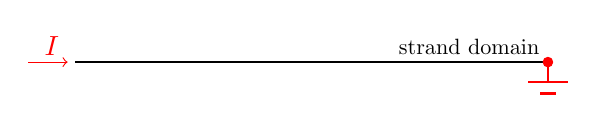
\begin{tikzpicture}[scale = 1]
\draw[thick, black] (-3,0) -- (3,0);
\filldraw[red] (3,0) circle (0.06);
\draw[thick, red] (3,0) -- (3,-0.25);
\draw[thick, red] (2.75,-0.25) -- (3.25,-0.25);
\draw[thick, red] (2.9,-0.4) -- (3.1,-0.4);
\draw[thin, red, ->] (-3.6,0) -- (-3.1,0);
\node[scale=0.8] at (2,0.2) {strand domain};
\node[scale=1.0, red] at (-3.3,0.2) {$I$};
\end{tikzpicture}
\caption{Electric boundary conditions.}
\label{fig: q_vel_benchmarking_electrical_settings}
\end{figure}

\begin{table}[h!]
    \caption{Analysis input parameters} 
    \vspace{-1.em} 
    \fontsize{10}{10}
    \selectfont 
    \renewcommand{\arraystretch}{1.5}
    \begin{center}
        \begin{tabular}{ ccc }  
        \hline
        $T_\text{init}$ & 1.9 & [K] \\
        $T_\text{max}$ & 20.0 & [K] \\
        $T_\text{c}$ & 8.429 & [K] \\
        $B$ & 2 & [T] \\
        $L_\text{quench, init}$ & 0.1 & [m] \\ 
        $\alpha$ & 0.223 & [m] \\   
        $I$ & 100 & [A] \\   
        RRR & 193 & [-] \\   
        f & 2.2 & [-] \\   
        time total & 0.1 & [s] \\   
        time step co-simulation & 0.0025 & [s] \\
        quench velocity & 6.81 & [m/s] \\
        \hline 
        \end{tabular}
    \end{center}  
     \label{table: 1d_qv_benchmarking_geometry_parameters_quench_velocity} 
 \end{table}
 
The aim of this analysis was to verify to what extent the nodal domain can be reduced as well as the time step might be increased while keeping the simulation error in an acceptable range. Two time step ranges in which ANSYS could choose step automatically were chosen: $t=\{[10, 100], [100, 1000]\}~\mu \text{s}$. Moreover, the simulation was conducted for 30, 50, 100, 500 and 1000 nodes along the one metre-long domain. 

Initial conditions related to temperature are similar to all previous analyses and are presented in Fig.~\ref{fig: init_gauss_temp_distr}. The analysis parameters are shown in Table \ref{table: 1d_qv_benchmarking_geometry_parameters_quench_velocity}. Many of them are repeated from the previous analyses. Based on standard benchmark solution from Section \ref{subsection:quench_velocity_benchmarking_no_insulation_heat_balance}, quench velocity is assumed to be constant. Time step co-simulation in Table  \ref{table: 1d_qv_benchmarking_geometry_parameters_quench_velocity} refers to time slots at which the external routine communicates with ANSYS in order to update the material properties in the model. The number of these slots equals 40. Such a high value serves for reducing calculation error due to the co-simulation itself.

\begin{figure}[h!]
\centering
    \begin{tikzpicture}
        \begin{axis}[
          no markers,
          width=0.7\linewidth, 
          height = 4.5cm,
          xlabel={$L_\text{strand},~\text{m}$},
          ylabel={$T,~\text{K}$},
          xmin=0.0,
          ymin=0.0,
          xmax=1.0
          ]
          
        %   Heat Balance Equation plots
          \addplot[red] table[x=position,y=t_0_03,col sep=comma] {sections/q_vel_modelling_benchmarking/figures/results_no_insulation/heat_balance_1000_nodes_benchmark.csv};
          \addplot[red] table[x=position,y=t_0_06,col sep=comma] {sections/q_vel_modelling_benchmarking/figures/results_no_insulation/heat_balance_1000_nodes_benchmark.csv};
          \addplot[red] table[x=position,y=t_0_1,col sep=comma] {sections/q_vel_modelling_benchmarking/figures/results_no_insulation/heat_balance_1000_nodes_benchmark.csv};

        %   Initial temperature curve for the mesh used in quench velocity modelling 
          \addplot[black] table[x=position,y=t_0,col sep=comma] {sections/q_vel_modelling_benchmarking/figures/results_no_insulation/quench_velocity_50_nodes_no_insulation.csv};

        %   Quench Velocity Modelling plots
          \addplot[blue] table[x=position,y=t_0_03,col sep=comma] {sections/q_vel_modelling_benchmarking/figures/results_no_insulation/quench_velocity_50_nodes_no_insulation.csv};
          \addplot[blue] table[x=position,y=t_0_06,col sep=comma] {sections/q_vel_modelling_benchmarking/figures/results_no_insulation/quench_velocity_50_nodes_no_insulation.csv};
          \addplot[blue] table[x=position,y=t_0_1,col sep=comma] {sections/q_vel_modelling_benchmarking/figures/results_no_insulation/quench_velocity_50_nodes_no_insulation.csv};
          
        \end{axis}
    \end{tikzpicture}
    \caption{Temperature distribution of a heat balance - based benchmark solution (in red) and a quench velocity - based solution (in blue) with 50 nodes along the domain for three time frames: $t=\{0.03, 0.06, 0.1\}$ s.}
    \label{fig: q_vel_benchmarking_temp_distr_over_strand_no_insulation}
\end{figure}

\begin{figure}[h!]
\centering
    \begin{tikzpicture}
        \begin{axis}[
          width=0.7\linewidth, 
          height = 4.5cm,
          xlabel={Time, $\text{s}$},
          ylabel={Resistive Voltage, $\text{V}$},
          xticklabel style={/pgf/number format/fixed},
          yticklabel style={/pgf/number format/fixed},
          xmin=0.0,
          xmax=0.1
          ]
          \addplot[blue, mark=*] table[x=time,y=50_nodes_quench_velocity,col sep=comma] {sections/q_vel_modelling_benchmarking/figures/results_no_insulation/quench_velocity_res_volt_benchmarking.csv};
          \addplot[red] table[x=time,y=heat_balance_benchmark,col sep=comma] {sections/q_vel_modelling_benchmarking/figures/results_no_insulation/quench_velocity_res_volt_benchmarking.csv};
        \end{axis}
    \end{tikzpicture}
    \caption{Resistive voltage comparison for standard numerical solution (in red) and quench velocity-based simulation with 50 nodes along the domain.}
    \label{fig: q_vel_modelling_res_volt_benchmarking}
\end{figure}

As presented in Fig. \ref{fig: q_vel_benchmarking_temp_distr_over_strand_no_insulation}, quench velocity - based co-simulation results in the quench front lagging behind the benchmark solution. The reasons standing behind this are the following: 
\begin{itemize}
    \item One can notice in Fig. \ref{fig:unidirectional_coupling_scheme} that the external routine updates resistive material properties at time slot $T_{j-1}$ and ANSYS solves the case for the time slot $T_{j}$. Therefore, the quenched zone is underestimated and 'delayed' with respect to standard quench numerical solution. To reduce this error, the number of co-simulation time slots was increased. 
    \item In quench velocity modelling, the material properties assignment to the strand is binary. The material has resistive materials of the strand composite above its critical temperature and no resistance below this value. The transition region of current sharing temperature is not taken into account. Therefore, the strand might not warm up sufficiently at the transition region.
\end{itemize}

However, the results important in the magnet design communities are: $(i)$ resistive voltage along the magnet coil, $(ii)$ hot spot temperature which is represented in this case at $x = 0~\text{m}$. As shown in Fig. \ref{fig: q_vel_modelling_res_volt_benchmarking}, the resistive voltage in quench velocity - based method follows the curve of the benchmark solution. In Fig. \ref{fig: q_vel_modelling_res_volt_rel_error}, one can notice that the relative error of the resistive voltage is also underestimated but converges to the range below -5\% for a relative extreme case of 50 nodes with respect to 1000 used for the heat balance equation - base benchmark solution. The relative error converges because the length of quench increases with time. Therefore, one can state that the longer the simulation lasts, the lower error is obtained. The relative error in case of the hot spot temperature did not exceed -2\% during the entire analysis and also converged to the value below -1\% as the simulation proceeded.

\begin{figure}[h!]
\centering
    \begin{tikzpicture}
        \begin{axis}[
          width=0.7\linewidth, 
          height = 4.5cm,
          xlabel={Time, $\text{s}$},
          ylabel={Relative error, \%},
          xticklabel style={/pgf/number format/fixed},
          xmin=0.0,
          xmax=0.1,
          legend pos=south east
          ]
          \addplot[blue, mark=*] table[x=time,y=50_nodes,col sep=comma] {sections/q_vel_modelling_benchmarking/figures/results_no_insulation/quench_velocity_res_volt_rel_error.csv};
          \addplot[red, mark=*] table[x=time,y=100_nodes,col sep=comma] {sections/q_vel_modelling_benchmarking/figures/results_no_insulation/quench_velocity_res_volt_rel_error.csv};
          \addplot[green, mark=*] table[x=time,y=1000_nodes,col sep=comma] {sections/q_vel_modelling_benchmarking/figures/results_no_insulation/quench_velocity_res_volt_rel_error.csv};
          \addlegendimage{/pgfplots/refstyle=plot_resistive_voltage}\addlegendentry{50 nodes}
          \addlegendimage{/pgfplots/refstyle=plot_resistive_voltage}\addlegendentry{100 nodes}
          \addlegendimage{/pgfplots/refstyle=plot_resistive_voltage}\addlegendentry{1000 nodes}
          
        \end{axis}
    \end{tikzpicture}
    \caption{Relative error of resistive voltage for 50, 100 and 1000 nodes used for quench velocity-based simulation.}
    \label{fig: q_vel_modelling_res_volt_rel_error}
\end{figure}

In Fig. \ref{fig: q_vel_modelling_res_volt_rel_error}, the case with 1000 nodes also shows the similar shape of the relative error curve. For that reason, the error cannot be explained by the decrease of mesh density since the benchmark standard numerical solution was of the same size. The error in the given range has to be accepted if one conducts the analyses using the quench velocity - based approach. In Table \ref{table: 1d_qv_benchmarking_no_insulation_methods_comparison}, the comparison of two methods is presented. With an accepted error of 5\%-10\%, the mesh size can be reduced from 10 to 20 times. What is also interesting, the solver converges to the solution with with 10 times larger time step. The quench velocity - based gave the results different by far less than 1\% when two different following time steps ranges were applied $t=\{[10, 100], [100, 1000]\}~\mu \text{s}$.

\begin{table}[h!]
    \caption{Methodology comparison} 
    \vspace{-1.em} 
    \fontsize{10}{10}
    \selectfont 
    \renewcommand{\arraystretch}{1.5}
    \begin{center}
        \begin{tabular}{ cccc }  
        \hline
          & mesh size & time step, $\mu \text{s}$ & simulation time, s\\
        \hline
        heat balance - based & 1000 & [10, 100] & 280 \\
        quench velocity - based & 50-100 & [100, 1000] & 280 \\
        \hline 
        improvement rate & 10-20 times & 10 times & none\\
        \end{tabular}
    \end{center}  
     \label{table: 1d_qv_benchmarking_no_insulation_methods_comparison} 
 \end{table}